\documentclass[aspectratio=169,12pt,xcolor=dvipsnames]{beamer}
\usepackage{graphicx} % For including graphics.
\usepackage{hyperref} % For links.
\usepackage{multirow}
\usepackage{minted}

\title{\Huge connascence}
\author{Jan Wedekind}
\date{Wednesday, April 9th 2025}

\hypersetup{
   pdftitle          = {connascence},
   pdfsubject        = {short presentation about connascence},
   pdfauthor         = {Jan Wedekind},
   pdfkeywords       = {software, quality, metric, engineering},
   pdfcreator        = {okular},
   pdfproducer       = {LaTeX with hyperref and thumbpdf},
   bookmarksopen     = false,
   bookmarksnumbered = true,
   colorlinks        = true,
}

\usebackgroundtemplate{
\includegraphics[width=\paperwidth,height=\paperheight]{slide}}

\usecolortheme{seahorse}

\definecolor{slidecolor}{rgb}{0.61,0.77,0.83}
\setbeamercolor{titlelike}{fg=black,bg=slidecolor!50}
\setbeamercolor{frametitle}{fg=black,bg=slidecolor!50}

\begin{document}

\begin{frame}
  \pdfbookmark[1]{connascence}{title}
  \titlepage
\end{frame}

\begin{frame}
  \pdfbookmark[1]{motivation}{motivation}
  \frametitle{motivation}
  \begin{itemize}
    \item metric for software design
    \item theoretical foundation for software engineering
  \end{itemize}
\end{frame}

\begin{frame}
  \pdfbookmark[1]{references}{references}
  \pdfbookmark[2]{Jim Weirich}{weirich}
  \frametitle{talk(s) by Jim Weirich}
  \begin{center}
    \href{https://www.youtube.com/watch?v=q85rdBMe9GY}{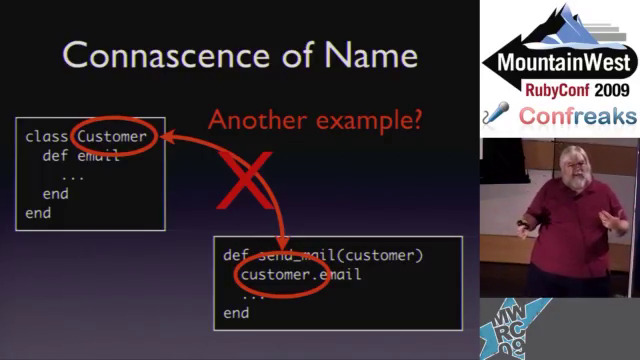
\includegraphics[height=.8\textheight]{weirich}}
  \end{center}
\end{frame}

\begin{frame}
  \pdfbookmark[2]{Meilir Page-Jones}{meilir}
  \frametitle{book by Meilir Page-Jones}
  \begin{center}
    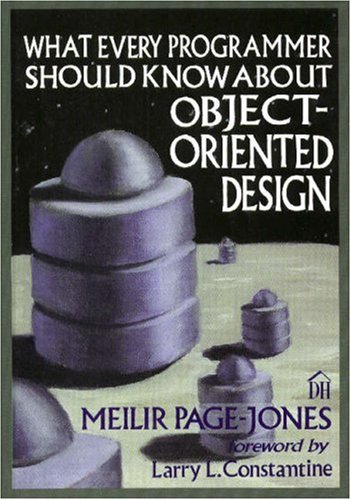
\includegraphics[height=.8\textheight]{meilir}
  \end{center}
\end{frame}

\begin{frame}
  \pdfbookmark[1]{definition}{definition}
  \frametitle{connascence definition}
  Jim Weirich:\bigskip\\
  \begin{quote}
    Two pieces of software share \textbf{connascence} when a change in one requires a corresponding change in the other.
  \end{quote}
\end{frame}

\begin{frame}
  \pdfbookmark[1]{kinds of connascence}{kinds}
  \frametitle{kinds of connascence ordered by increasing strength}
  \begin{center}
    \begin{tabular}{|l|l|l|}\hline
      & \textbf{abbreviation}  & \textbf{kind} \\\hline
      \multirow{5}{*}{static}  & \textbf{CoN}  & Connascence of Name\\
      & \textbf{CoT}  & Connascence of Type\\
      & \textbf{CoM}  & Connascence of Meaning\\
      & \textbf{CoP}  & Connascence of Position\\
      & \textbf{CoA}  & Connascence of Algorithm\\\hline
      \multirow{4}{*}{dynamic} & \textbf{CoE}  & Connascence of Execution\\
      & \textbf{CoTi} & Connascence of Timing\\
      & \textbf{CoV}  & Connascence of Value\\
      & \textbf{CoI}  & Connascence of Identity\\\hline
    \end{tabular}\\\bigskip
    Also see \url{https://connascence.io/}
  \end{center}
\end{frame}

\begin{frame}[fragile]
  \pdfbookmark[1]{examples}{examples}
  \pdfbookmark[2]{CoN}{con}
  \frametitle{connascence of name (CoN)}
  \begin{center}
    \begin{minipage}[c]{.35\textwidth}
      \begin{minted}[bgcolor=black!10]{python}
def sqr(x):
    return x
      \end{minted}
    \end{minipage}
    \begin{minipage}[c]{.35\textwidth}
      \begin{minted}[bgcolor=black!10]{python}
l = sqr(x) + sqr(y)
      \end{minted}
    \end{minipage}
  \end{center}
\end{frame}

\begin{frame}[fragile]
  \pdfbookmark[2]{CoT}{cot}
  \frametitle{connascence of type (CoT)}
  \begin{center}
    \begin{minipage}[c]{.65\textwidth}
      \begin{minted}[bgcolor=black!10]{python}
from datetime import datetime

def date_to_isostring(date: datetime):
    return date.strftime('%Y-%m-%d')
      \end{minted}
    \end{minipage}
    \begin{minipage}[c]{.65\textwidth}
      \begin{minted}[bgcolor=black!10]{python}
date_to_isostring(datetime(2025, 4, 2))
      \end{minted}
    \end{minipage}
  \end{center}
\end{frame}

\begin{frame}[fragile]
  \pdfbookmark[2]{CoM}{com}
  \frametitle{connascence of meaning (CoM)}
  \begin{center}
    \begin{minipage}[c]{.5\textwidth}
      \begin{minted}[bgcolor=black!10]{python}
class Order:
    def ship_order(self):
        self.status = 2
      \end{minted}
    \end{minipage}
    \begin{minipage}[c]{.5\textwidth}
      \begin{minted}[bgcolor=black!10]{python}
if order.status == 2:
    print('Order was shipped.')
      \end{minted}
    \end{minipage}
  \end{center}
\end{frame}

\begin{frame}[fragile]
  \pdfbookmark[2]{CoP}{cop}
  \frametitle{connascence of position (CoP)}
  \begin{center}
    \begin{minipage}[c]{.5\textwidth}
      \begin{minted}[bgcolor=black!10]{python}
def imwrite(filename, image):
    # ...
      \end{minted}
    \end{minipage}
    \begin{minipage}[c]{.5\textwidth}
      \begin{minted}[bgcolor=black!10]{python}
imwrite('image.jpg', image)
      \end{minted}
    \end{minipage}
  \end{center}
\end{frame}

\begin{frame}[fragile]
  \pdfbookmark[2]{CoA}{coa}
  \frametitle{connascence of algorithm (CoA)}
  \begin{center}
    \begin{minipage}[c]{.98\textwidth}
      \begin{minted}[bgcolor=black!10]{python}
from werkzeug.security import generate_password_hash

hashed_password = generate_password_hash(password)
      \end{minted}
    \end{minipage}
    \begin{minipage}[c]{.98\textwidth}
      \begin{minted}[bgcolor=black!10]{python}
from werkzeug.security import check_password_hash

is_correct = check_password_hash(hashed_password, user_input)
      \end{minted}
    \end{minipage}
  \end{center}
\end{frame}

\begin{frame}[fragile]
  \pdfbookmark[2]{CoE}{coe}
  \frametitle{connascence of execution (CoE)}
  \begin{center}
    \begin{minipage}[c]{.6\textwidth}
      \begin{minted}[bgcolor=black!10]{python}
email = Email()
email.set_recipient('foo@example.com')
email.set_sender('me@mydomain.com')
email.send()
email.set_subject('Hello World')
      \end{minted}
    \end{minipage}
  \end{center}
\end{frame}

\begin{frame}
  \pdfbookmark[2]{CoTi}{coti}
  \pdfbookmark[2]{CoV}{cov}
  \pdfbookmark[2]{CoI}{coi}
  \frametitle{other kinds of connascence}
  \begin{center}
    \begin{tabular}{|ll|p{.55\textwidth}|}\hline
      connascence of timing   & (CoTi) & The timing of the execution of multiple components is important.\\\hline
      connascence of value    & (CoV)  & Several values must change together.\\\hline
      connascence of identity & (CoI)  & Multiple components must reference the same entity.\\\hline
    \end{tabular}
  \end{center}
\end{frame}

\begin{frame}
  \pdfbookmark[1]{properties}{properties}
  \frametitle{properties of connascence}
  \begin{center}
    \begin{tabular}{|l|p{.55\textwidth}|}\hline
      \textbf{strength} & Difficulty of refactoring associated with each kind of connascence.\\\hline
      \textbf{locality} & Closeness of the involved entities (same method, same class, same module, ...).\\\hline
      \textbf{degree}   & Number of entities involved in an instance of connascence.\\\hline
    \end{tabular}
  \end{center}
\end{frame}

% examples of code transformation to a kind of connascence with reduced strength

% https://www.wedesoft.de/downloads/connascence.pdf

\end{document}
